% ONE SESSION, TWO PEOPLE. The wearer's exposure to the carried load is the
% binding constraint on the whole design, so it gets its own track and its
% own annotation; the operator's fatigue is a different process and is drawn
% separately rather than pooled.
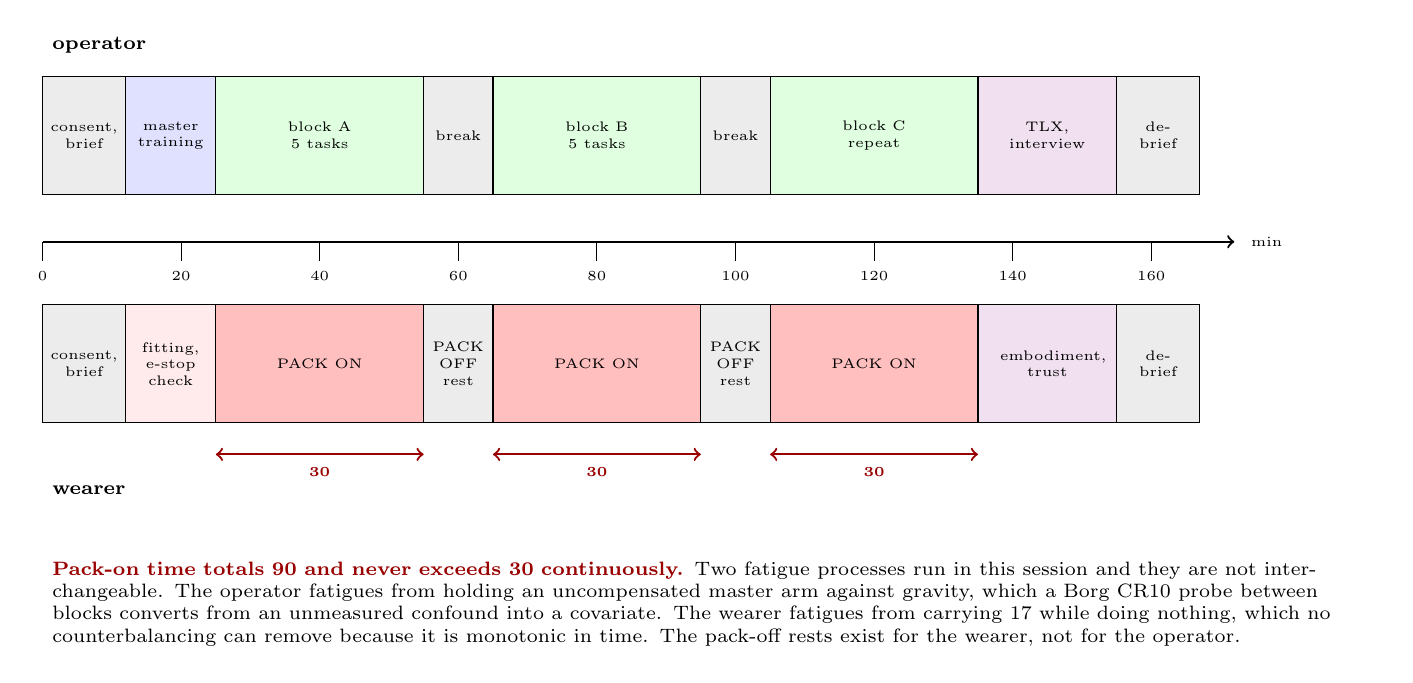
\begin{tikzpicture}[x=0.88mm, y=1mm, font=\scriptsize]

\draw[->, thick] (0,0) -- (172,0);
\node[font=\tiny, anchor=west] at (173,0) {min};
\foreach \t in {0,20,...,160} \draw (\t,0) -- (\t,-2.5)
  node[below, font=\tiny] {\t};

\node[anchor=west, font=\bfseries\scriptsize] at (0, 25) {operator};
\foreach \a/\b/\c/\l in {0/12/gray!15/{consent,\\brief},
                         12/25/blue!12/{master\\training},
                         25/55/green!12/{block A\\5 tasks},
                         55/65/gray!15/{break},
                         65/95/green!12/{block B\\5 tasks},
                         95/105/gray!15/{break},
                         105/135/green!12/{block C\\repeat},
                         135/155/violet!12/{TLX,\\interview},
                         155/167/gray!15/{de-\\brief}}
{
  \pgfmathsetmacro{\m}{(\a+\b)/2}
  \draw[fill=\c] (\a,6) rectangle (\b,21);
  \node[align=center, text width=12mm, font=\tiny] at (\m,13.5) {\l};
}

\node[anchor=west, font=\bfseries\scriptsize] at (0, -31.5) {wearer};
\foreach \a/\b/\c/\l in {0/12/gray!15/{consent,\\brief},
                         12/25/red!8/{fitting,\\e-stop check},
                         25/55/red!25/{PACK ON},
                         55/65/gray!15/{PACK OFF\\rest},
                         65/95/red!25/{PACK ON},
                         95/105/gray!15/{PACK OFF\\rest},
                         105/135/red!25/{PACK ON},
                         135/155/violet!12/{embodiment,\\trust},
                         155/167/gray!15/{de-\\brief}}
{
  \pgfmathsetmacro{\m}{(\a+\b)/2}
  \draw[fill=\c] (\a,-23) rectangle (\b,-8);
  \node[align=center, text width=12mm, font=\tiny] at (\m,-15.5) {\l};
}

\foreach \a/\b in {25/55, 65/95, 105/135}
  \draw[<->, thick, red!60!black] (\a,-27) -- (\b,-27)
     node[midway, below=1pt, font=\tiny\bfseries, red!60!black] {\SI{30}{\minute}};

\node[anchor=west, font=\scriptsize, text width=168mm, align=left]
  at (0, -46)
  {\textbf{\color{red!60!black}Pack-on time totals \SI{90}{\minute} and never
   exceeds \SI{30}{\minute} continuously.} Two fatigue processes run in this
   session and they are not interchangeable. The operator fatigues from
   holding an uncompensated master arm against gravity, which a Borg CR10
   probe between blocks converts from an unmeasured confound into a covariate.
   The wearer fatigues from carrying \SI{17}{\kilo\gram} while doing nothing,
   which no counterbalancing can remove because it is monotonic in time. The
   pack-off rests exist for the wearer, not for the operator.};
\end{tikzpicture}
